\documentclass[a4paper,11pt]{book}
\usepackage{import}
\usepackage{preamb}

\makeindex

\begin{document}

\small
\begin{multicols}{3}

%\maketitle

\thispagestyle{empty}
\scriptsize
\newpage


\begin{subbox}{subbox}{}
\centering
\Large{\textbf{Network Science   \\ Cheatsheet}}
\end{subbox}

\begin{multibox}{2}
\begin{subbox}{subbox}{}
\centering

\includegraphics[width=0.8\textwidth]{pics/logo.png}
\end{subbox}
\begin{subbox}{subbox}{}
\centering
Made by \\
\large{
Remy Cazabet
}
\end{subbox}
\end{multibox}
% \section{Blocks and Community structure}


\begin{subbox}{subbox}{}
\centering
\Large{\textbf{Assortativity}}
\end{subbox}




\begin{textbox}{Assortativity - Homophily - Mixing Patterns}

A network is said to be \textbf{assortative} or to demonstrate \textbf{homophily} if its nodes tend to connect more with other nodes that are \textbf{similar} than to nodes that are different. 

Similarity in this case must be understood in term of nodes properties. Some typical examples can be age, gender, language, political beliefs, etc.

Homophily is considered a common feature of many networks, in particular social networks\footcite{mcpherson2001birds}, as reflected in the aphorism \textit{Birds of a feather flock together}.

Typical examples would be \textit{age, gender, ethnicity} or \textit{politicla opinions} in social networks networks such as Twitter \footcite{mcpherson2001birds}
\end{textbox}





\begin{textbox}{Disassortativity - Heterophily}
Some networks can also demonstrate \textbf{heterophily}, or \textbf{disassortativity}, i.e., a greater number of connections with nodes that are different (for instance, in a sentimental relationship network, women tend to connect more with men than with other women, and reciprocally).
\end{textbox}


\begin{textbox}{Mixing Patterns}
The notion of nodes connecting to each other with preferences based on their attributes can be generalized to the concept of \textbf{Mixing Patterns}. Beyond homophily/heterophily, nodes with property $p_1$ can be preferentially connected to nodes with property $p_2$ (and not $p_3$ or $p_4$) while nodes having property $p_3$ can have a preference for nodes having the same property, for instance.


\end{textbox}


\begin{textbox}{Mixing Patterns - example}
Example of mixing patterns of age in the Pokec\footnote{https://snap.stanford.edu/data/soc-pokec.html} social  network. Better examples of rich mixing patterns can be found in \footcite{del2007mixing}.

\centering

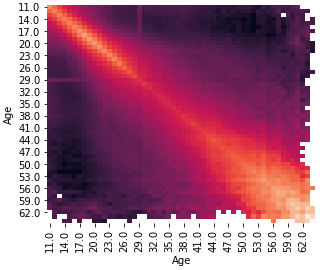
\includegraphics[width=0.9\textwidth]{pics/mixing_patterns.png}

We can see that there is some level of assortativity (high values on the diagonal), but that there are also some more complex mixing patterns, for instance between age 10 and 40, approximately, here interpreted as child-parents relationships.

\end{textbox}



\begin{textbox}{Note on interpreting homophily}
Homophily can be a link creation mechanism (nodes have a preference to connect with similar ones, so the network end up to be assortative), or a consequence of influence phenomenons (because nodes are connected, they tend to influence each other and thus become more similar).

Without access to the dynamic of the network and its properties, it is not possible to differentiate those effects.
\end{textbox}





\begin{textbox}{Categorical or Numerical homophily}

Attributes of nodes can be either categorical (no natural order between values, discrete number of possible values), or numerical (natural order, discrete or continuous). Although the general idea remains the same, the way to compute homophily differs according to type of attributes we are interested in.
\end{textbox}






\begin{textbox}{Assortativity Index - Definition}
When the property for which we study homophily is \textbf{categorical}, homophily can be defined\footcite{newman2003mixing} by comparing the fraction of edges that connect nodes of the same category, and the expected value of such edges if the network was random. More formally, it is expressed as:

\[
r=\frac{\sum_i e_{ii} - \sum_i a_i^2}{1- \sum_i a_i^2}
\]
where $e_ii$ is the fraction of edges connecting two nodes of category $i$, and $a_i$ the fraction of all edges connected to a node of category $i$ (sum of degrees divided by number of edges).
\end{textbox}




\begin{textbox}{Assortativity index - Example}

Let's see a fictional example of how to compute the assortativity index. Nodes are individuals, edges represent for instance some social interaction. Columns/Rows correspond to blood types, and numbers are expressed in fraction of the total number of edges.

\centering
\begin{tabular}{|
>{\columncolor[HTML]{EFEFEF}}l |
>{\columncolor[HTML]{FFFFFF}}l 
>{\columncolor[HTML]{FFFFFF}}l 
>{\columncolor[HTML]{FFFFFF}}l 
>{\columncolor[HTML]{FFFFFF}}l 
>{\columncolor[HTML]{EFEFEF}}l |}
\hline
Blood Types & \multicolumn{1}{l|}{\cellcolor[HTML]{EFEFEF}A} & \multicolumn{1}{l|}{\cellcolor[HTML]{EFEFEF}AB} & \multicolumn{1}{l|}{\cellcolor[HTML]{EFEFEF}B} & \multicolumn{1}{l|}{\cellcolor[HTML]{EFEFEF}O} & $a_i$        \\ \hline
A           & \cellcolor[HTML]{ECF4FF}0.30                   & 0.05                                            & 0.1                                            & 0.05                                           & \textit{0.5} \\ \cline{1-1}
AB          & 0.05                                           & \cellcolor[HTML]{ECF4FF}0.05                    & 0                                              & 0                                              & \textit{0.1} \\ \cline{1-1}
B           & 0.1                                            & 0                                               & \cellcolor[HTML]{ECF4FF}0.2                    & 0                                              & \textit{0.3} \\ \cline{1-1}
O           & 0.05                                           & 0                                               & 0                                              & \cellcolor[HTML]{ECF4FF}0.05                   & \textit{0.1} \\ \cline{1-1}
$a_i$      & \cellcolor[HTML]{EFEFEF}\textit{0.5}           & \cellcolor[HTML]{EFEFEF}\textit{0.1}            & \cellcolor[HTML]{EFEFEF}\textit{0.3}           & \cellcolor[HTML]{EFEFEF}\textit{0.1}           & \textbf{1}   \\ \hline
\end{tabular}

\vspace{0.3cm}

$r=\frac{(0.3+0.05+0.2+0.05)-(0.5^2+0.1^2+0.3^2+0.1^2)}{1-(0.5^2+0.1^2+0.3^2+0.1^2)}=\frac{0.6+0.36}{1-0.36}=0.375$
\end{textbox}























\begin{textbox}{Asortativity index - Properties}

An assortativity index of $r=0$ means that the network has no assortative mixing, $r=1$ corresponds to a perfectly assortative network (edges exist only between nodes of the same category), and $r=-1$ to a perfectly disassortative network (no edge between nodes of the same category).
\end{textbox}




\begin{textbox}{Assortativity and Modularity}

Assortativity is related to the Modularity, a measure of the quality of \textit{communities}, by the following relation:

\[
r=\frac{Q}{Q_{max}}
\]
Indeed, $\sum_i e_{ii} - \sum_i a_i^2$ corresponds to the definition of the Modularity, while $1- \sum_i a_i^2$ corresponds to the maximal value that the Modularity could reach if all nodes were in the same communities.
\end{textbox}








\begin{textbox}{Homophily for numeric variables}
When the property for which we study homophily is \textbf{numeric}, homophily $r$ can be defined as the \textbf{Pearson Correlation Coefficient} between values at both end of each edge. For details, see \cite{newman2003mixing}.

\end{textbox}




\begin{textbox}{Numeric Assortativity index - Properties}

Homophily $r=0$ means that the network has no assortative mixing, $r>0$ corresponds to an assortative network (nodes with high values tend to connect to high values), and $r<0$ to a disassortative network (nodes with high values are preferably connected to low values).

\end{textbox}








\begin{textbox}{Degree assortativity}
\textbf{Degree assortativity}\footcite{newman2003mixing}, sometimes simply called \textit{assortativity}, is a particular case of homophily measured  in term of node degrees, i.e., the numerical value associated to each node is its degree.

The existence of a degree assortativity can be interpreted in term of a \textit{rich club phenomenon}: hubs prefer to connect to other hubs.

ER, Configuration and BA random graph models have a degree assortativity equals to 0, while many real networks have positive values, and some negative ones.

\end{textbox}




\begin{textbox}{Limits of Assortativity}
A limit of assortativity coefficients as we have defined them is that they summarize the whole network as a single value. However, different parts of the network might have different types of assortativity. For instance, the 3 following graphs have a similar value of assortativity ($\approx 0$).

\centering

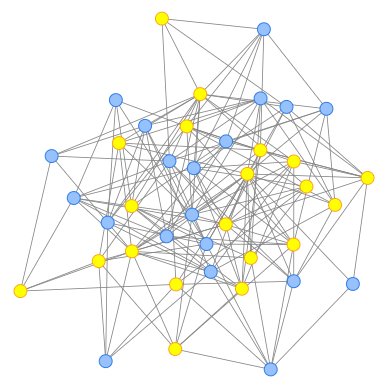
\includegraphics[width=0.30\textwidth]{pics/asso1.png}
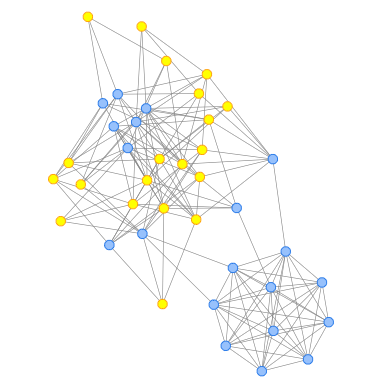
\includegraphics[width=0.30\textwidth]{pics/asso2.png}
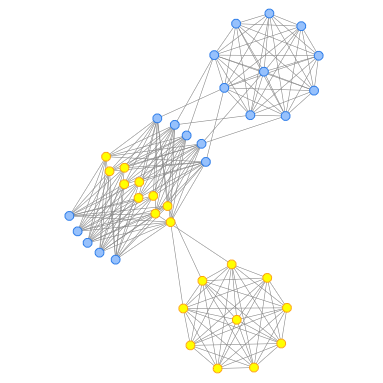
\includegraphics[width=0.30\textwidth]{pics/asso3.png}


Figure inspired from \footcite{peel2018multiscale}, in which the authors propose a local measure of \textbf{multiscale assortativity}. Another longer distance assortativity is defined in .
\end{textbox}


\begin{textbox}{Going Further}
\begin{itemize}
    \item A survey on the topic (\cite{noldus2015assortativity})
    \item Non-local assortativity (\cite{peel2018multiscale}) (\cite{rossetti2021conformity})
\end{itemize}

\end{textbox}


% \begin{textbox}{Neighbor connectivity }
% \textbf{Neighbor connectivity} is another way to study the correlation between node degrees. The principle is to study how the degree of nodes relates to the average degree of its neighbors, i.e., the relation between $k_u$ and \frac{1}{|N_u|}$\sum_{v\in N_u} k_v$ for all $u$. The sign of the correlation between those variables inform about the 

%%%% Be careful, check the relation with the friendship paradox
% \end{textbox}

 \AtNextBibliography{\footnotesize}


\printbibliography[heading=subbibliography]


\end{multicols}



\end{document}


